\section{Results}
\label{sec:results}

Table~\ref{tab:bench_main} gives the test ROC-AUC of every model under every protocol on both datasets, and Figure~\ref{fig:bench} shows the same numbers with their intervals. Every paired comparison with \kaam{} is listed in Appendix~\ref{app:more}.

% Generated by scripts/paper_tables.py. Do not edit.
\begin{table*}[t]
\centering
\footnotesize
\setlength{\tabcolsep}{3.5pt}
\TabCaption{tab:bench_main}{Test ROC-AUC of every model under every protocol}{Mean over test sets (five splits or folds where applicable) of the mean over seeds, with the 95\% bootstrap interval below (tasks resampled; users for the user-grouped protocol). Bold: best model in the column of each panel. $^{\circ}$: the difference from \kaam{} is not significant after Holm correction. Intervals resample test tasks with the fitted models held fixed, so they do not include training or fold variation. Under the protocols the EBMs were fitted on the original sample only (compute; Appendix~\ref{app:deviations}).}
\begin{tabular}{@{}lccccccc@{}}
\toprule
Model & \begin{tabular}[b]{@{}c@{}}Random\end{tabular} & \begin{tabular}[b]{@{}c@{}}Time,\\all users\end{tabular} & \begin{tabular}[b]{@{}c@{}}Time,\\known users\end{tabular} & \begin{tabular}[b]{@{}c@{}}Time,\\new users\end{tabular} & \begin{tabular}[b]{@{}c@{}}User-\\grouped\end{tabular} & \begin{tabular}[b]{@{}c@{}}Without\\User~1\end{tabular} & \begin{tabular}[b]{@{}c@{}}Without\\Users~1,~4\end{tabular} \\
\midrule
\multicolumn{8}{@{}l}{\emph{Full trace (\V{data.full.tasks} tasks)}} \\
KAAM & 0.766 & 0.594 & 0.596 & 0.466 & \textbf{0.641} & 0.703 & 0.672 \\
 & {\tiny [0.764, 0.767]} & {\tiny [0.589, 0.599]} & {\tiny [0.591, 0.601]} & {\tiny [0.424, 0.508]} & {\tiny [0.527, 0.670]} & {\tiny [0.698, 0.709]} & {\tiny [0.665, 0.678]} \\[1pt]
Logistic regression & 0.732 & 0.576 & 0.580 & 0.462$^{\circ}$ & 0.600 & 0.656 & 0.630 \\
 & {\tiny [0.730, 0.734]} & {\tiny [0.571, 0.581]} & {\tiny [0.574, 0.585]} & {\tiny [0.420, 0.504]} & {\tiny [0.491, 0.633]} & {\tiny [0.650, 0.662]} & {\tiny [0.623, 0.637]} \\[1pt]
MLP & 0.804 & 0.596$^{\circ}$ & \textbf{0.599}$^{\circ}$ & 0.482$^{\circ}$ & 0.637$^{\circ}$ & 0.721 & 0.698 \\
 & {\tiny [0.802, 0.805]} & {\tiny [0.592, 0.601]} & {\tiny [0.594, 0.604]} & {\tiny [0.445, 0.521]} & {\tiny [0.539, 0.664]} & {\tiny [0.716, 0.726]} & {\tiny [0.692, 0.704]} \\[1pt]
LightGBM & \textbf{0.900} & \textbf{0.599}$^{\circ}$ & \textbf{0.599}$^{\circ}$ & \textbf{0.534} & 0.566$^{\circ}$ & \textbf{0.845} & \textbf{0.805} \\
 & {\tiny [0.899, 0.901]} & {\tiny [0.594, 0.604]} & {\tiny [0.594, 0.604]} & {\tiny [0.496, 0.573]} & {\tiny [0.520, 0.599]} & {\tiny [0.841, 0.849]} & {\tiny [0.799, 0.810]} \\[1pt]
\midrule
\multicolumn{8}{@{}l}{\emph{Original sample (\V{data.orig.tasks} tasks)}} \\
KAAM & 0.744 & 0.595 & 0.603 & 0.515 & \textbf{0.620} & 0.698 & 0.627 \\
 & {\tiny [0.735, 0.754]} & {\tiny [0.572, 0.618]} & {\tiny [0.579, 0.629]} & {\tiny [0.423, 0.605]} & {\tiny [0.551, 0.641]} & {\tiny [0.667, 0.728]} & {\tiny [0.591, 0.665]} \\[1pt]
Logistic regression & 0.723 & 0.588$^{\circ}$ & 0.589$^{\circ}$ & \textbf{0.565}$^{\circ}$ & 0.561$^{\circ}$ & 0.662 & 0.602 \\
 & {\tiny [0.713, 0.732]} & {\tiny [0.561, 0.614]} & {\tiny [0.561, 0.618]} & {\tiny [0.458, 0.666]} & {\tiny [0.487, 0.601]} & {\tiny [0.632, 0.693]} & {\tiny [0.563, 0.640]} \\[1pt]
MLP & 0.722 & 0.523 & 0.533 & 0.548$^{\circ}$ & 0.540 & 0.681$^{\circ}$ & 0.531 \\
 & {\tiny [0.714, 0.729]} & {\tiny [0.499, 0.547]} & {\tiny [0.507, 0.558]} & {\tiny [0.462, 0.628]} & {\tiny [0.486, 0.564]} & {\tiny [0.652, 0.709]} & {\tiny [0.516, 0.544]} \\[1pt]
LightGBM & \textbf{0.810} & \textbf{0.619}$^{\circ}$ & \textbf{0.620}$^{\circ}$ & 0.552$^{\circ}$ & 0.502$^{\circ}$ & \textbf{0.756} & 0.673 \\
 & {\tiny [0.801, 0.818]} & {\tiny [0.595, 0.642]} & {\tiny [0.595, 0.647]} & {\tiny [0.461, 0.640]} & {\tiny [0.469, 0.577]} & {\tiny [0.728, 0.784]} & {\tiny [0.642, 0.706]} \\[1pt]
EBM, additive & 0.756 & 0.595$^{\circ}$ & 0.596$^{\circ}$ & 0.533$^{\circ}$ & 0.489$^{\circ}$ & 0.722 & 0.646 \\
 & {\tiny [0.746, 0.765]} & {\tiny [0.571, 0.620]} & {\tiny [0.572, 0.621]} & {\tiny [0.423, 0.636]} & {\tiny [0.454, 0.588]} & {\tiny [0.693, 0.752]} & {\tiny [0.611, 0.682]} \\[1pt]
EBM, pairwise & 0.803 & 0.573$^{\circ}$ & 0.565$^{\circ}$ & 0.539$^{\circ}$ & 0.504$^{\circ}$ & 0.752 & \textbf{0.685} \\
 & {\tiny [0.794, 0.811]} & {\tiny [0.545, 0.601]} & {\tiny [0.535, 0.596]} & {\tiny [0.430, 0.641]} & {\tiny [0.466, 0.599]} & {\tiny [0.724, 0.781]} & {\tiny [0.650, 0.720]} \\[1pt]
\bottomrule
\end{tabular}
\TabNotes
\end{table*}


\begin{figure*}[t]
\centering
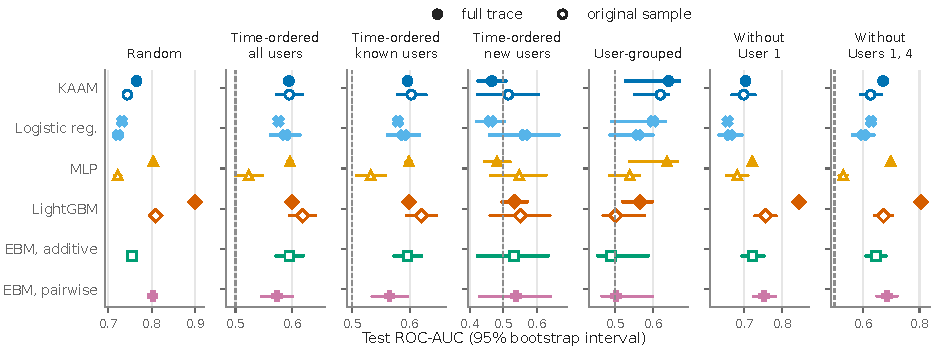
\includegraphics[width=\textwidth]{figures/benchmark.pdf}
\caption{Test ROC-AUC with 95\% bootstrap intervals for every model and protocol; filled markers: full trace, open markers: original sample. The EBMs were fitted on the original sample only. Dashed line: chance. Each panel has its own horizontal scale.}
\label{fig:bench}
\end{figure*}

\subsection{Random splits}
\label{sec:res-random}

On the full trace \kaam{} reaches \V{full.random.kaam.auc} \V{full.random.kaam.ci}. It is above logistic regression by \V{full.random.lr.diff} (\V{full.random.lr.dci}, \V{full.random.lr.sig}) and below the parameter-matched MLP by \V{full.random.mlp.absdiff} (\V{full.random.mlp.dci}) and LightGBM by \V{full.random.lgbm.absdiff} (\V{full.random.lgbm.dci}); both differences are \V{full.random.lgbm.sig}. On the original sample, where all six models were fitted, \kaam{} reaches \V{orig.random.kaam.auc}: above logistic regression (\V{orig.random.lr.diff}) and the MLP (\V{orig.random.mlp.diff}), slightly below the additive EBM (\V{orig.random.ebm.diff}, \V{orig.random.ebm.dci}), and well below the two models with interactions, LightGBM (\V{orig.random.lgbm.diff}) and the EBM with pairwise terms (\V{orig.random.ebmi.diff}). All five differences are \V{orig.random.lgbm.sig} after Holm correction, and none lies within the $\pm$\V{stat.margin} margin, so \kaam{} matches none of the baselines. The two additive models are close to each other and the two models with interactions are close to each other, with a gap of about \V{orig.random.ebmi.absdiff} between the pairs. The MLP is weaker on the original sample than in the first version (\V{orig.random.mlp.auc} over five splits, against \V{v1.mlp.auc} on one split there); the first version's best learning rate is not in the present grid, and the networks now stop on validation AUC. The spread between splits is small next to these gaps (\kaam{}: standard deviation \V{orig.random.kaam.setstd} over the five splits of the original sample and \V{full.random.kaam.setstd} on the full trace).

\paragraph{Exact duplicates.} In each random split of the full trace, \V{rf.full.dup.random.min} to \V{rf.full.dup.random.max} of the test tasks have an exact copy of all ten raw features among the training tasks: concurrent submissions of the same request that land on the same machine within the same window. Under the time-ordered split the share is \V{rf.full.dup.time.max}, in the user-grouped folds \V{rf.full.dup.grouped.min} to \V{rf.full.dup.grouped.max}, and in the original sample, which samples the trace sparsely, \V{rf.orig.dup.random.min} to \V{rf.orig.dup.random.max}. A random split of the full trace therefore rewards recognising duplicated requests as well as known users. The larger random-split score of LightGBM on the full trace than on the original sample (\V{full.random.lgbm.auc} against \V{orig.random.lgbm.auc}) is consistent with this, although we did not separate the two effects. This check was added after an independent review.

\paragraph{Calibration.} PR-AUC and the Brier score order the models as ROC-AUC does (Table~\ref{tab:calib_full}). Under the random protocol LightGBM, the MLP and \kaam{} are close to calibrated on the full trace (ECE \V{full.random.lgbm.ece}, \V{full.random.mlp.ece} and \V{full.random.kaam.ece}), and logistic regression is less so (\V{full.random.lr.ece}; Figure~\ref{fig:reliability}). Under the time-ordered and user-grouped protocols the base rate of the test tasks differs from that of the training tasks, and calibration degrades (ECE \V{full.time.minece} to \V{full.time.maxece} and \V{full.grouped.minece} to \V{full.grouped.maxece}).

% Generated by scripts/paper_tables.py. Do not edit.
\begin{table}[t]
\centering
\small
\setlength{\tabcolsep}{3pt}
\TabCaption{tab:calib_full}{Precision-recall and calibration, full trace}{PR-AUC is average precision; Brier score and expected calibration error (ECE, 15 equal-width bins) are lower-is-better. Means over test sets and seeds.}
\begin{tabular}{@{}lccccccccc@{}}
\toprule
 & \multicolumn{3}{c}{Random} & \multicolumn{3}{c}{Time, all} & \multicolumn{3}{c}{User-grouped} \\
\cmidrule(lr){2-4}\cmidrule(lr){5-7}\cmidrule(lr){8-10}
Model & PR-AUC & Brier & ECE & PR-AUC & Brier & ECE & PR-AUC & Brier & ECE \\
\midrule
KAAM & 0.641 & 0.149 & 0.034 & 0.211 & 0.142 & 0.069 & 0.355 & 0.172 & 0.112 \\
Logistic regression & 0.546 & 0.165 & 0.084 & 0.191 & 0.141 & 0.066 & 0.336 & 0.182 & 0.133 \\
MLP & 0.685 & 0.136 & 0.018 & 0.211 & 0.139 & 0.056 & 0.370 & 0.173 & 0.105 \\
LightGBM & 0.849 & 0.093 & 0.017 & 0.196 & 0.139 & 0.051 & 0.304 & 0.183 & 0.105 \\
\bottomrule
\end{tabular}
\TabNotes
\end{table}


\begin{figure*}[t]
\centering
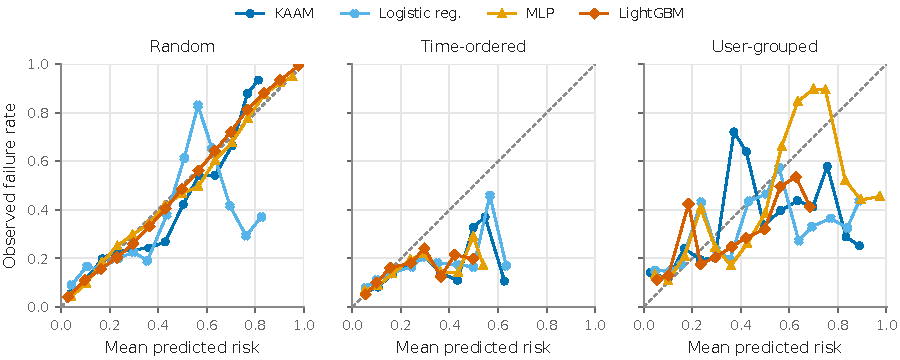
\includegraphics[width=\textwidth]{figures/reliability.pdf}
\caption{Reliability diagrams on the full trace (first seed, test sets of a protocol pooled, bins with at least \V{fig.minbin} tasks). Dashed: perfect calibration.}
\label{fig:reliability}
\end{figure*}

\subsection{Time-ordered split}
\label{sec:res-time}

Training on the first \V{prot.time.train} of the full trace by start time and testing on the last \V{prot.time.test}, which spans \V{full.split.time.t.testdays} days, every model drops to between \V{full.time.minauc} and \V{full.time.maxauc}. \kaam{} reaches \V{full.time.kaam.auc} \V{full.time.kaam.ci} and LightGBM \V{full.time.lgbm.auc} \V{full.time.lgbm.ci}; their difference is \V{full.time.lgbm.sig}. The drop is not an effect of new users: \V{full.split.time.t.knownshare} of the test tasks come from users with training tasks, and on those tasks the models score between \V{full.timeknown.minauc} and \V{full.timeknown.maxauc}. The \V{full.split.time.t.newn} test tasks of new users are scored between \V{full.timenew.minauc} and \V{full.timenew.maxauc} (\kaam{}: \V{full.timenew.kaam.auc} \V{full.timenew.kaam.ci}). The period matters more than the user here. The validation period, the \V{prot.time.val} of tasks just before the test period, is a burst dominated by User~1, who submits \V{rf.full.time.val.u1} of its tasks against \V{rf.full.time.train.u1} of the training tasks and \V{rf.full.time.test.u1} of the test tasks. Its failure rate is \V{full.split.time.t.rateval} (\V{rf.full.time.val.rateno1} without User~1), against \V{full.split.time.t.ratetrain} in training and \V{full.split.time.t.ratetest} in test, and on it the same models reached validation AUCs between \V{full.time.minvalauc} and \V{full.time.maxvalauc}; the networks stopped after about \V{full.time.mlp.bestepoch} epochs (MLP) and \V{full.time.kaam.bestepoch} (\kaam{}). Model selection on this period overstated the accuracy in the test week, which starts \V{rf.full.time.gap} days after the last training task. The \V{full.split.time.t.newn} new-user test tasks come from \V{rf.full.time.newusers} users; on them LightGBM is the best model, above \kaam{} by \V{full.timenew.lgbm.absdiff} (\V{full.timenew.lgbm.sig} under the task-level bootstrap, which treats these tasks as independent although they come from few users). The original sample shows the same pattern (Table~\ref{tab:bench_main}).

\subsection{User-grouped folds}
\label{sec:res-grouped}

With users held out, the full-trace AUCs fall to between \V{full.grouped.minauc} and \V{full.grouped.maxauc} (Table~\ref{tab:grouped_full}, Figure~\ref{fig:folds}). The five folds are unequal. StratifiedGroupKFold places User~1 with two small users in fold~\V{full.mech.u1fold}, whose \V{full.mech.u1.ntest} test tasks come from \V{full.mech.u1.testusers} users, so that fold is in effect a test on User~1 alone and its user-level interval rests on three clusters; the other folds hold \V{full.mech.nou.min.users} to \V{full.mech.nou.max.users} test users each. On those \V{full.gnou.nfolds} folds the mean AUCs are \V{full.gnou.mlp.auc} for the MLP, \V{full.gnou.kaam.auc} for \kaam{}, \V{full.gnou.lr.auc} for logistic regression and \V{full.gnou.lgbm.auc} for LightGBM; on the fold with User~1 they are \V{full.gu1.kaam.auc}, \V{full.gu1.mlp.auc}, \V{full.gu1.lr.auc} and \V{full.gu1.lgbm.auc} for \kaam{}, the MLP, logistic regression and LightGBM. Over all five folds \kaam{} has the highest mean, \V{full.grouped.kaam.auc} \V{full.grouped.kaam.ci}, but its differences from the MLP (\V{full.grouped.mlp.diff}, \V{full.grouped.mlp.dci}) and from LightGBM (\V{full.grouped.lgbm.diff}, \V{full.grouped.lgbm.dci}) are not significant, the interval of the difference with the MLP extends past the $\pm$\V{stat.margin} margin on both sides, and the ranking depends on how the folds are combined. No model is clearly best on new users. LightGBM's grouped fits stopped early: their mean best iteration ranges from \V{full.lgbm.grouped.minrounds} to \V{full.lgbm.grouped.maxrounds} boosting rounds over the folds, against \V{full.lgbm.random.minrounds} to \V{full.lgbm.random.maxrounds} on the random splits, and its seed-to-seed spread is \V{full.grouped.lgbm.seedstd} against \V{full.grouped.kaam.seedstd} for \kaam{}. Its low grouped score reflects ensembles that early stopping on validation users cut almost at once; a more strongly regularised or interaction-constrained boosting model was not tested. On the original sample \kaam{} leads on the \V{orig.gnou.nfolds} folds without User~1 (\V{orig.gnou.kaam.auc} against \V{orig.gnou.min} to \V{orig.gnou.lr.auc} for the other models), on about three thousand test tasks per fold. Against chance, \V{full.chance.nsig} of the \V{full.chance.nmodels} full-trace models and \V{orig.chance.nsig} of the \V{orig.chance.nmodels} original-sample models are significantly above 0.5 after Holm correction, and none is significantly below it. Fold AUCs on the full trace range from \V{full.fold.minauc} to \V{full.fold.maxauc}, and \V{full.fold.nbelow} of the \V{full.fold.npairs} fold-model pairs fall below 0.5.

% Generated by scripts/paper_tables.py. Do not edit.
\begin{table*}[t]
\centering
\footnotesize
\setlength{\tabcolsep}{3pt}
\TabCaption{tab:grouped_full}{User-grouped folds on the full trace}{AUC per fold (mean over seeds), the fold mean with a user-level bootstrap interval and its Holm-adjusted $p$-value against 0.5, and the one-core mechanism per fold.}
\begin{tabular}{@{}lcccccccc@{}}
\toprule
Model & Fold 0 & Fold 1 & Fold 2 & Fold 3 & Fold 4 & Mean & 95\% CI & $p_{\mathrm{Holm}}$ vs.\ 0.5 \\
\midrule
KAAM & 0.581 & 0.551 & 0.559 & 0.760 & 0.754 & 0.641 & [0.527, 0.670] & 0.014 \\
Logistic regression & 0.586 & 0.496 & 0.486 & 0.782 & 0.651 & 0.600 & [0.491, 0.633] & 0.095 \\
MLP & 0.563 & 0.540 & 0.595 & 0.799 & 0.686 & 0.637 & [0.539, 0.664] & 0.004 \\
LightGBM & 0.522 & 0.574 & 0.626 & 0.490 & 0.616 & 0.566 & [0.520, 0.599] & 0.006 \\
\midrule
Test users & 288 & 278 & 277 & 313 & 3 &  &  &  \\
Test tasks & 86,778 & 86,746 & 86,800 & 86,745 & 192,747 &  &  &  \\
One-core failure rate, train & 82.5\% & 77.1\% & 82.6\% & 78.2\% & 19.5\% &  &  &  \\
Other failure rate, train & 20.4\% & 20.5\% & 20.6\% & 19.0\% & 19.5\% &  &  &  \\
One-core failure rate, test & 27.8\% & 36.5\% & 15.0\% & 16.3\% & 87.2\% &  &  &  \\
Other failure rate, test & 17.4\% & 17.3\% & 18.1\% & 23.1\% & 20.6\% &  &  &  \\
AUC of $-$\feat{plan_cpu}, train & 0.734 & 0.728 & 0.727 & 0.694 & 0.559 &  &  &  \\
AUC of $-$\feat{plan_cpu}, test & 0.455 & 0.474 & 0.431 & 0.717 & 0.765 &  &  &  \\
\bottomrule
\end{tabular}
\TabNotes
\end{table*}


\begin{figure}[t]
\centering
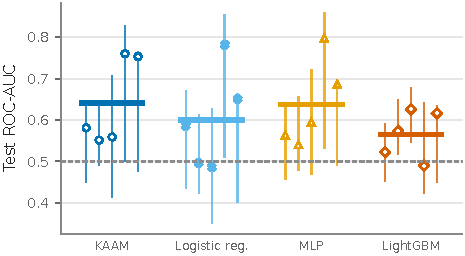
\includegraphics[width=0.62\linewidth]{figures/grouped_folds.pdf}
\caption{User-grouped folds on the full trace. Open markers: AUC of each fold (mean over seeds) with its user-level 95\% interval; bar: mean over folds. Dashed line: chance.}
\label{fig:folds}
\end{figure}

\paragraph{Why some folds fall below chance.} In every training split that contains User~1, one-core tasks fail at \V{rf.oc.with.minone} to \V{rf.oc.with.maxone} against \V{rf.oc.with.minother} to \V{rf.oc.with.maxother} for other tasks, and User~1 holds \V{rf.oc.with.minu1} to \V{rf.oc.with.maxu1} of the one-core training tasks. Without User~1 the difference almost disappears: one-core tasks fail at \V{rf.oc.groupedf4.one} against \V{rf.oc.groupedf4.other} among the training users of fold~\V{full.mech.u1fold}, and at \V{rf.oc.louod1.one} against \V{rf.oc.louod1.other} in the split without User~1. Among the held-out users of the other folds the picture is mixed (Table~\ref{tab:grouped_full}, lower rows): one-core tasks fail more often than other tasks in folds~0 and~1 (\V{full.mech.f0.teonerate} and \V{full.mech.f1.teonerate} against \V{full.mech.f0.teotherrate} and \V{full.mech.f1.teotherrate}) and less often in folds~2 and~3 (\V{full.mech.f2.teonerate} and \V{full.mech.f3.teonerate} against \V{full.mech.f2.teotherrate} and \V{full.mech.f3.teotherrate}). Ranking all test tasks by $-$\feat{plan_cpu}, the direction the models learn, gives AUCs of \V{full.mech.nou.min.teauc} to \V{full.mech.nou.max.teauc} on the held-out users, below chance in \V{full.mech.nou.nrev} of these folds: a rule learned largely from User~1 overstates the one-core risk of most other users and orders their larger requests poorly.

\subsection{Leaving out the dominant users}
\label{sec:res-louo}

Removing every task of User~1 changes the test population as well as the training data: User~1's tasks fail at \V{users.full.u1.rate} against \V{users.full.nonu1.rate} for the other users, and their presence makes ranking easier. The AUCs of this protocol are therefore not directly comparable with those of the random protocol, and the protocol does not separate the effect of User~1 on training from its effect on the test set. Without User~1, and without Users~1 and~4, LightGBM still leads \kaam{} by \V{full.louoa.lgbm.absdiff} and \V{full.louob.lgbm.absdiff} (both \V{full.louob.lgbm.sig}). Its random-split lead is therefore not explained by the two dominant users; the exact duplicates described above, \V{rf.full.dup.louo.min} to \V{rf.full.dup.louo.max} of the test tasks of these splits, are one candidate.

\subsection{Interpretability}
\label{sec:res-interp}

\paragraph{The contributions are exact SHAP values.} Kernel SHAP with every one of the \V{shap.coalitions} feature coalitions, a background of \V{shap.background} training tasks and \V{shap.tasks} test tasks returns the centred \kaam{} contributions of the canonical model to within \V{shap.maxdiff} log-odds, and the ten contributions plus the bias reproduce the model's logit to within \V{shap.sumgap}. No sampling enters a \kaam{} explanation; the same holds for any additive model, the additive EBM included, so this property does not favour the KAN parameterisation over other additive models.

\paragraph{The curves.} Figure~\ref{fig:curves} shows the ten curves of the canonical model for its five seeds, with the corresponding curve of the original sample. The five seeds give nearly identical curves. Validation chose no smoothness penalty on all five random splits of the full trace, and the strongest value, \V{model.lambdamax}, on the time-ordered split and on \V{full.lambda.grouped.em2} of the five user-grouped folds, where the validation tasks come from a later period or from other users. On the random splits the four request features therefore get curves that oscillate between the few values that occur (the ticks in Figure~\ref{fig:curves}); such a curve is informative only at observed values. The telemetry curves are smooth: risk rises with the recent kernel CPU of the machine and falls steeply as its recent load rises from low values, the pattern the first version reported and attributed, tentatively, to the trace recording telemetry mostly for workers that finished.

\begin{figure*}[t]
\centering
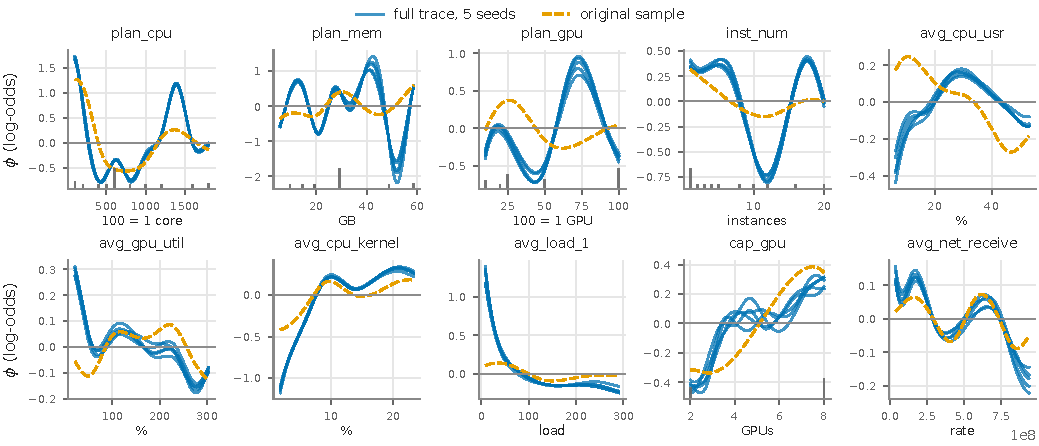
\includegraphics[width=\textwidth]{figures/curves_all.pdf}
\caption{The ten curves of the canonical \kaam{} (full trace, random split \V{prot.canon}) for five seeds, and the curve learned on the original sample (dashed), each centred on its mean over the training 5th to 95th percentile. Ticks: values of the discrete features held by at least \V{fig.tickshare} of training tasks, with height proportional to their share.}
\label{fig:curves}
\end{figure*}

\paragraph{\kaam{} against the additive EBM.} The two additive models fit their shape functions in different ways, B-splines by gradient descent and piecewise-constant terms by cyclic boosting, so their agreement is a check on both (Table~\ref{tab:shapecorr}, Figure~\ref{fig:shapes}). On the grid fixed in the protocol the median correlation over the ten features is \V{ebm.r.median}; the telemetry curves agree closely, while two request features show almost no agreement (lowest: \V{ebm.r.worstfeat}, $r=\V{ebm.r.min}$). Evaluated at the training tasks' own values, an exploratory measure not fixed in the protocol, the median correlation is \V{ebm.rd.median} and the lowest \V{ebm.rd.min} (\V{ebm.rd.worstfeat}). The disagreement is therefore concentrated between observed values of the discrete requests, where neither model has data. On the canonical split the additive EBM, fitted once on the full trace, reaches a test AUC of \V{full.s42.ebm.auc} against \V{full.s42.kaam.auc} for \kaam{}.

% Generated by scripts/paper_tables.py. Do not edit.
\begin{table}[t]
\centering
\small
\TabCaption{tab:shapecorr}{\kaam{} and additive EBM shape functions}{$r_{\mathrm{grid}}$: Pearson correlation of the two centred curves on 200 evenly spaced points between the training 5th and 95th percentiles, as fixed in the protocol. $r_{\mathrm{data}}$ (exploratory): the same correlation at the values of up to \V{ebm.rd.ntasks} training tasks inside that window, so that each value counts as often as it occurs; for the request features, which take few distinct values, the grid version mostly compares how the two models fill the gaps between observed values. Swing: maximum minus minimum of each curve over the window, in log-odds. Canonical random split of the \V{ebm.shapeds}, seed~0.}
\begin{tabular}{@{}lcccc@{}}
\toprule
Feature & $r_{\mathrm{grid}}$ & $r_{\mathrm{data}}$ & \kaam{} swing & EBM swing \\
\midrule
\feat{plan_mem} & 0.04 & 0.75 & 3.16 & 2.97 \\
\feat{plan_cpu} & 0.62 & 0.99 & 2.50 & 2.62 \\
\feat{plan_gpu} & 0.04 & 0.57 & 1.66 & 0.97 \\
\feat{avg_load_1} & 0.97 & 0.97 & 1.61 & 1.79 \\
\feat{avg_cpu_kernel} & 0.98 & 0.99 & 1.47 & 1.71 \\
\feat{inst_num} & 0.46 & 0.81 & 1.22 & 1.17 \\
\feat{cap_gpu} & 0.70 & 1.00 & 0.76 & 0.68 \\
\feat{avg_cpu_usr} & 0.90 & 0.88 & 0.54 & 0.64 \\
\feat{avg_gpu_util} & 0.85 & 0.82 & 0.43 & 0.45 \\
\feat{avg_net_receive} & 0.80 & 0.76 & 0.29 & 0.47 \\
\bottomrule
\end{tabular}
\TabNotes
\end{table}


\begin{figure*}[t]
\centering
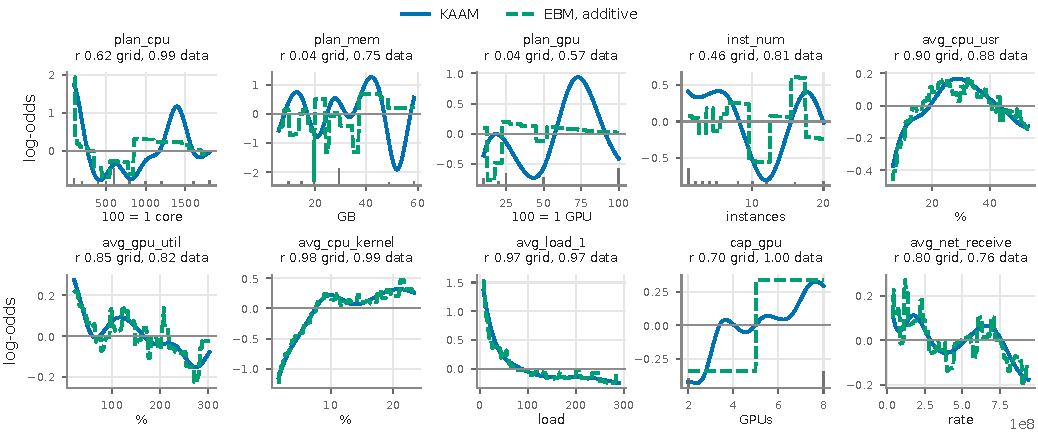
\includegraphics[width=\textwidth]{figures/shapes_kaam_ebm.pdf}
\caption{Shape functions of \kaam{} and of the additive EBM on the canonical split, centred on their means over the training 5th to 95th percentile. Panel titles give the correlation on the protocol's evenly spaced grid and at the training tasks' values. Ticks as in Figure~\ref{fig:curves}.}
\label{fig:shapes}
\end{figure*}

\paragraph{The one-core curve under each protocol.} Figure~\ref{fig:plancpu} overlays the \feat{plan_cpu} curve of the first seed under every protocol of the full trace. On the canonical split the centred curve stands at \V{pc.randoms42.onecore} log-odds at one core. With User~1 removed it stands at \V{pc.louod1.onecore}, and with Users~1 and~4 removed at \V{pc.louod14.onecore}. In the user-grouped folds the value at one core ranges from \V{pc.grouped.minone} to \V{pc.grouped.maxone}; the lowest is fold~\V{full.mech.u1fold}, whose training set also lacks User~1. A centred value reflects the whole shape of a curve as well as the one-core effect, and the shape changes from fit to fit (correlation with the canonical curve between \V{pc.groupedf1.corr} and \V{pc.groupedf0.corr} over the grouped folds, \V{pc.timet.corr} for the time-ordered split), so the training data give the clearer evidence: with User~1 in training, one-core tasks fail at \V{rf.oc.with.minone} to \V{rf.oc.with.maxone} against \V{rf.oc.with.minother} to \V{rf.oc.with.maxother} for other tasks, and without User~1 at \V{rf.oc.groupedf4.one} against \V{rf.oc.groupedf4.other} (fold~\V{full.mech.u1fold}) and \V{rf.oc.louod1.one} against \V{rf.oc.louod1.other} (split without User~1). Centring on the mean training task instead of the grid, a post hoc check, a one-core request adds \V{ph.oc.randoms42} log-odds on the canonical split and \V{ph.oc.gwith.min} to \V{ph.oc.gwith.max} in the grouped folds whose training users include User~1, against \V{ph.oc.louod1} without User~1 and \V{ph.oc.louod14} without Users~1 and~4. Fold~\V{full.mech.u1fold}, trained without User~1, still gives \V{ph.oc.gwithout}, although its one-core and other training tasks fail at \V{ph.oc.gwithout.trone} and \V{ph.oc.gwithout.trother}. The curves are a complete account of each fitted model; they are not a stable account of the data. A second rise near thirteen cores appears with and without User~1 but not in the time-ordered curve.

\begin{figure}[t]
\centering
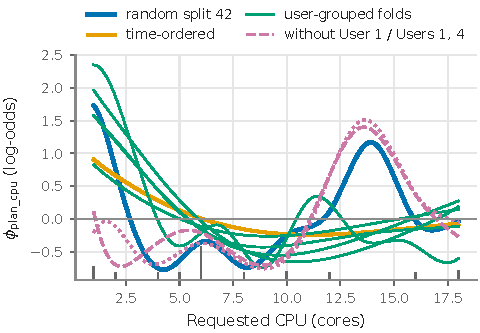
\includegraphics[width=0.62\linewidth]{figures/plan_cpu_protocols.pdf}
\caption{The \feat{plan_cpu} curve of \kaam{} (first seed) under each protocol of the full trace, centred on the same window. Ticks: request values held by at least \V{fig.tickshare} of the canonical training tasks.}
\label{fig:plancpu}
\end{figure}

\subsection{Case audits}
\label{sec:res-cases}

The four cases were selected on the canonical model's test set by the rule fixed in the first version: the most confident true positive and true negative, and the false negative and false positive with the highest risk at a threshold of 0.5 (Table~\ref{tab:cases}, Figure~\ref{fig:waterfall}). Each bar is the contribution of one feature relative to the mean training task, whose logit is \V{case.baselogit}; in every case the ten contributions and the bias reproduce the logit to within \V{case.maxsumgap}.

The true positive (risk \V{case.tp.risk}) is a one-core request, and \feat{plan_cpu} contributes \V{case.tp.c.plancpu}, \V{case.tp.topshare} of the total absolute push. The identical four-field request occurs in \V{case.tp.samereq} training tasks, \V{case.tp.samerate} of which failed and \V{case.tp.sameu1} of which came from User~1. The false positive (risk \V{case.fp.risk}) is also a one-core request and receives the same \V{case.fp.c.plancpu} from \feat{plan_cpu}, plus \V{case.fp.c.planmem} from a large memory request. Its own request occurs in only \V{case.fp.samereq} training tasks, \V{case.fp.samerate} of which failed and none from User~1: the one-core term learned largely from one user's recurring job is applied to another user's task. The false negative (risk \V{case.fn.risk}, just below the threshold) requests half a core (\V{case.fn.c.plancpu}) and \V{case.fn.raw.instnum} instances (\V{case.fn.c.instnum}); its request occurs in \V{case.fn.samereq} training tasks with a failure rate of \V{case.fn.samerate}. The true negative (risk \V{case.tn.risk}) owes most of its score to \feat{plan_gpu} at the \V{case.tn.pct.plangpu} percentile (\V{case.tn.c.plangpu}); its exact request occurs in \V{case.tn.samereq} training tasks, none of which failed. A confident score that rests on a sparse region of one feature is visible at a glance in this form.

% Generated by scripts/paper_tables.py. Do not edit.
\begin{table*}[t]
\centering
\small
\TabCaption{tab:cases}{Four case audits of the canonical \kaam{}}{Selected by the rule fixed in advance (most confident true positive and true negative; highest-risk false negative and false positive at threshold 0.5). Contributions are log-odds relative to the mean training task. Same request: training tasks with the identical four resource requests / their failure rate / the share submitted by User~1.}
\begin{tabular}{@{}lcp{7.2cm}l@{}}
\toprule
Case & Risk & Largest three contributions & Same request \\
\midrule
True positive & 0.861 & \feat{plan_cpu} +1.68; \feat{avg_load_1} +0.41; \feat{avg_cpu_kernel} +0.36 & 44,191 / 87\% / 100\% \\
True negative & 0.002 & \feat{plan_gpu} $-$4.32; \feat{plan_cpu} $-$0.80; \feat{cap_gpu} $-$0.50 & 18 / 0\% / 0\% \\
False negative & 0.500 & \feat{plan_cpu} +1.60; \feat{inst_num} $-$0.86; \feat{cap_gpu} +0.22 & 1,995 / 5\% / 0\% \\
False positive & 0.878 & \feat{plan_cpu} +1.68; \feat{plan_mem} +0.79; \feat{avg_cpu_kernel} +0.26 & 44 / 5\% / 0\% \\
\bottomrule
\end{tabular}
\TabNotes
\end{table*}


\begin{figure*}[t]
\centering
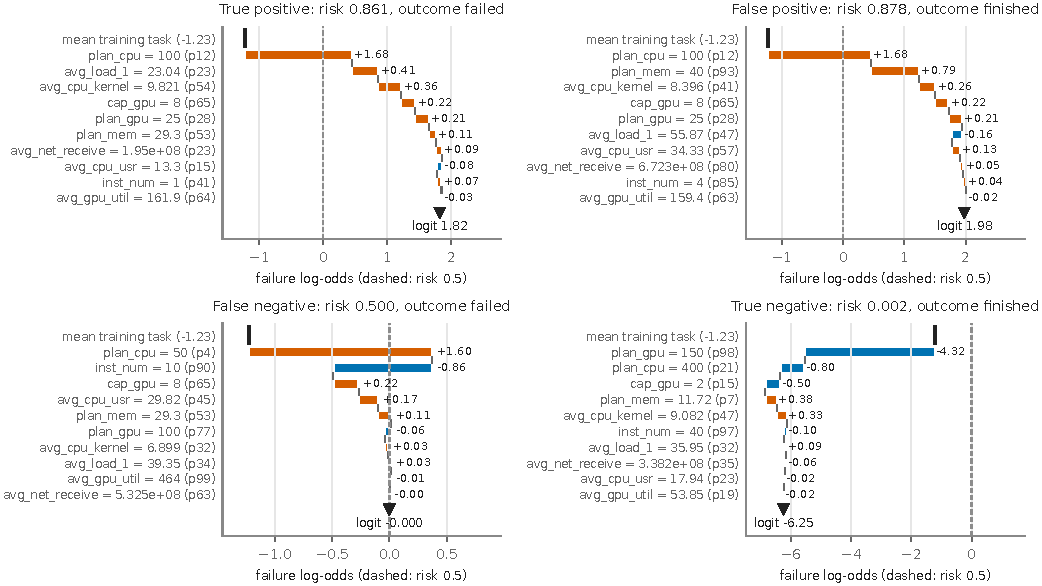
\includegraphics[width=\textwidth]{figures/case_waterfall.pdf}
\caption{Case audits of the canonical \kaam{}. Each panel runs from the logit of the mean training task (top) through the ten contributions, largest first, to the model's logit (bottom). The mean training task's logit is the bias plus each contribution's mean over training tasks. Labels give the raw value and its percentile among training tasks (pNN); the dashed line is risk 0.5.}
\label{fig:waterfall}
\end{figure*}

\subsection{Lookback window}
\label{sec:res-lookback}

On the original sample each window keeps the split roles of the one-hour build, and \kaam{} is refitted for each window (Table~\ref{tab:lookback}, Figure~\ref{fig:lookback}). On the test tasks scored at both widths, the windows of \V{lb.wide} score between \V{lb.2.diff} and \V{lb.6.diff} AUC above the one-hour model, and the half-hour window differs from it by \V{lb.0p5.diff}; after Holm correction \V{lb.nsig} of the four differences is significant, and none exceeds \V{lb.maxabsdiff}. The one-hour window is a reasonable default, and the conclusions do not depend on it.

% Generated by scripts/paper_tables.py. Do not edit.
\begin{table}[t]
\centering
\small
\setlength{\tabcolsep}{3pt}
\TabCaption{tab:lookback}{Lookback window ablation on the original sample}{Each window keeps the canonical 1\,h split roles of its tasks. Own AUC: on the window's own test set. $\Delta$: AUC minus the 1\,h model on the test tasks both score, with the paired 95\% interval; $p$ is Holm-adjusted over the four windows. \kaam{}, seed~0.}
\begin{tabular}{@{}lrrcrcc@{}}
\toprule
Window & Tasks & Test & Own AUC & Shared & $\Delta$ [95\% CI] & $p_{\mathrm{Holm}}$ \\
\midrule
0.5\,h & 17,751 & 2,671 & 0.760 & 2,671 & 0.000 [$-$0.002, 0.002] & 0.707 \\
1\,h & 18,890 & 2,834 & 0.753 & -- & reference & -- \\
2\,h & 19,524 & 2,930 & 0.753 & 2,834 & +0.003 [0.001, 0.005] & 0.032 \\
4\,h & 19,911 & 2,988 & 0.752 & 2,834 & +0.004 [0.001, 0.007] & 0.069 \\
6\,h & 20,067 & 3,011 & 0.750 & 2,834 & +0.004 [0.000, 0.008] & 0.069 \\
\bottomrule
\end{tabular}
\TabNotes
\end{table}


\begin{figure}[t]
\centering
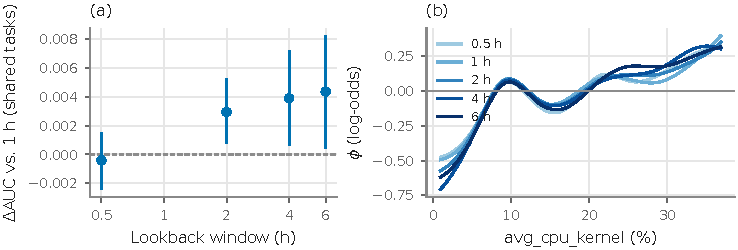
\includegraphics[width=0.85\linewidth]{figures/lookback.pdf}
\caption{Lookback ablation on the original sample. (a) AUC of each window minus the one-hour model on the test tasks both score, with paired 95\% intervals. (b) The \feat{avg_cpu_kernel} curve at each window.}
\label{fig:lookback}
\end{figure}

